\documentclass{standalone}
\usepackage{tikz}
\usepackage{ctex,siunitx}
\setCJKmainfont{Noto Serif CJK SC}
\usepackage{tkz-euclide}
\usepackage{amsmath}
\usetikzlibrary{patterns, calc,3d}
\usetikzlibrary {decorations.pathmorphing,decorations.pathreplacing,decorations.shapes}
\begin{document}
\small
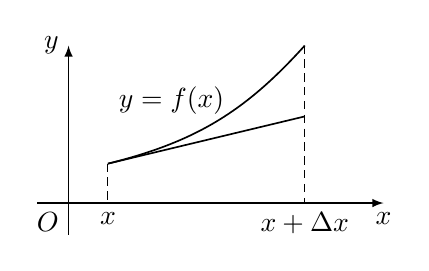
\begin{tikzpicture}[>=latex,scale=1.0]
  \draw[->](-0.4,0)--(4,0)node[below]{$x$};
  \draw[->](0,-0.4)--(0,2)node[left]{$y$};
  \node at (0,0)[below left]{$O$};
  \draw[densely dashed](0.5,0.5)--(0.5,0)node[below]{$x$};
  \draw[densely dashed](3.0,2.0)--(3.0,0)node[below]{$x+\Delta x$};
  \draw[semithick](0.5,0.5)--(3.0,1.1);
  \draw[semithick](0.5,0.5)to[bend right=17](3.0,2.0);
  \node at (2.1,1.3)[left]{$y=f(x)$};
\end{tikzpicture}
\end{document}